\documentclass{report}
\usepackage[T1]{fontenc}
\usepackage[utf8]{inputenc}
\usepackage[francais]{babel}
\usepackage{amsmath}
\usepackage{graphicx}
\graphicspath{{Figures/}}
\usepackage[backend=biber,style=authoryear,bibencoding=utf8]{biblatex}
\usepackage[colorlinks,linkcolor=blue]{hyperref}
\newcommand{\micro}{$\mathrm{\mu}$}
\addbibresource{biblio.bib}

\begin{document}

\chapter{Rhéologie cellulaire}

L'étude des propriétés mécaniques des objets biologiques (cellules, tissus, gels de biopolymères \dots) a été investie par des physiciens convergeant à la fois de la mécanique des milieux continus, de la physique de la matière molle (polymères, mousses, colloïdes, verres), et de l'hydrodynamique. 
En effet, ils rassemblent des objets et des propriétés qui intéressent tous ces domaines, à d'une échelle moléculaire à une échelle macroscopique. 

Il est aisé de voir à quelle point la mécanique peut être un aspect important du vivant : les médecins détectent les anomalies d'un tissu en testant sa rigidité \og à la main \fg pendant une palpation, l'absence de gravité a des conséquences importantes sur les os, et l'absence d'exercice sur les muscles, tandis que les changements de propriétés mécaniques des globules rouges ou des parois des vaisseaux sanguins peuvent se révéler dramatiques. 

Les matériaux vivants, comme les tendons, les os ou la cornée, ou issus du vivant comme la soie ou la nacre peuvent également posséder des propriétés rhéologiques intéressantes, que l'on cherche à dupliquer pour créer de nouveaux matériaux composites. 

Les matériaux vivants combinent plusieurs particularités qui en font des objets particulièrement difficiles à étudier du point de vue physique : ils sont intrinsèquement hors de l'équilibre thermodynamique, car ils consomment de l'énergie en permanence, ils ne sont le plus souvent ni homogènes, ni isotropes, sont composés d'une grande diversité de constituants différents, leurs propriétés varient à la fois au cours du temps et d'un individu à l'autre. 
Tous ces éléments rendent plus complexes la reproductibilité d'une mesure à l'autre, la comparaison de mesures prises par des techniques différentes, l'élaboration de modèles théoriques et de simulations numériques.


\section{Rhéologie}

La rhéologie est l'étude de la manière dont les matériaux se comportent lorsqu'ils sont soumis à une contrainte mécanique.

Par exemple, on appelle solide élastique un matériau pour lequel la déformation $\epsilon$ à un étirement uniaxial est proportionnelle à la contrainte $ \sigma$, et on appelle module d'Young ce coefficient de proportionnalité : 
$$ E = \frac{\sigma}{\epsilon}$$
La déformation élastique est parfaitement réversible, c'est-à-dire que si on enlève la contrainte, le matériau revient à sa forme initiale. C'est le cas, aux petites déformations, de solides comme l'acier, le verre, le caoutchouc etc. Au niveau énergétique, la déformation élastique est donc une manière de stocker de l'énergie dans le système par l'intermédiaire de la déformation, énergie qui pourra être récupérée plus tard lorsque le solide reprendra sa forme initiale. 

\begin{figure}
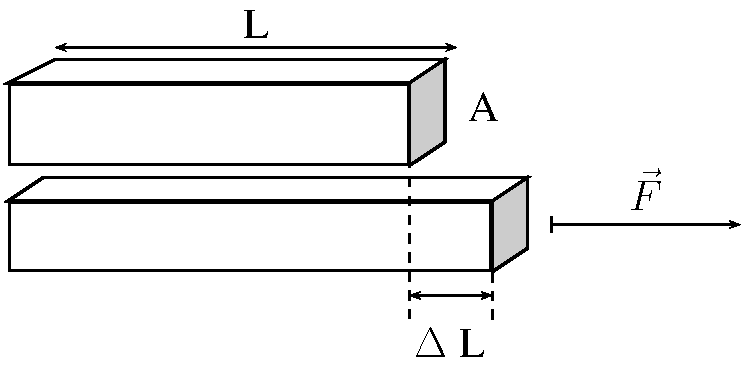
\includegraphics[scale=0.5]{Figures/Young_modulus.pdf} 
\caption{Solide élastique de section $A$ soumis à une contrainte $\sigma=\frac{F}{A}$ et déformé de $\epsilon=\frac{\Delta L}{L}$.  }
\end{figure}

Au contraire, pour les liquides visqueux, la viscosité $\eta$ représente la relation entre la contrainte et le taux de déformation $\dot{\epsilon}$ : 
$$ \eta=\frac{\sigma}{\dot{\epsilon}}$$
Le liquide va donc être déformé de manière linéaire au cours du temps sous l'effet d'une contrainte constante. Lorsque que la contrainte est levée, la déformation s'arrête, mais le liquide ne reprend pas la forme qu'il avait avant son application. 
L'écoulement visqueux est un phénomène irréversible, et l'énergie qui a été fournie pour le faire s'écouler est dissipée. 

Le liquide purement visqueux et le solide purement élastique sont des modèles qui ne sont valables que dans certaines limites. Une barre d'acier est élastique dans une gamme de contraintes et de déformations, au-delà elle est plastique : elle se déforme de manière irréversible en réponse à la contrainte. 
Cela peut également dépendre de l'échelle de temps à laquelle on se place, par exemple, le manteau de la croûte terrestre peut être considéré comme un solide élastique à une échelle de temps de quelques heures, mais à des échelles de temps géologiques, il peut être considéré comme un liquide extrêmement visqueux ($\eta \approx 10^{21}$Pa.s). 


La fonction de fluage quantifie la déformation d'un matériau en réponse à une contrainte $\sigma$ constante appliquée à partir d'un temps $t=0$. 
Dans le cas simple du solide élastique, la fonction de fluage est une constante : à l'application d'une contrainte, le matériau est immédiatement déformé, et cette déformation reste constante par la suite. Par exemple, dans le cas d'un étirement uniaxial : 
$$J(t)=\frac{1}{E}$$
Dans le cas d'un liquide visqueux cisaillé, la fonction de fluage est une fonction linéaire du temps : 
$$ J(t)=\frac{t}{\eta}$$

Les cellules vivantes et la plupart des bio-polymères sont des matériaux visco-élastiques, ce qui signifie qu'une partie de l'énergie transmise par la contrainte va être stockée, et une autre va être dissipée. Il existe plusieurs manières simples de combiner les deux modèles précédents pour créer un modèle de visco-élasticité. 

Les deux plus simples sont le modèle de Kelvin-Voigt et le modèle de Maxwell, qui associent un élément élastique de module d'Young $E$ et un élément visqueux de viscosité $\eta$, le premier en parallèle et le second en série. 
Dans le modèle de Maxwell, lorsque l'on impose une contrainte $\sigma$ constante, on obtient une superposition des deux fonctions de fluage précédentes : 
$$J(t)=\frac{1}{E} + \frac{t}{\eta} = \frac{1}{E} \left( 1 + \frac{t}{\tau} \right) \qquad \tau= \frac{\eta}{E}$$ 
et donc une déformation affine au cours du temps. Le matériau se déforme de manière élastique, puis coule en relaxant la contrainte. 
Dans le modèle de Kelvin-Voigt : 
$$ J(t)=\frac{1}{E} e^{-\frac{t}{\tau}} \qquad \tau=\frac{\eta}{E}$$
Un temps caractéristique du système apparaît, en dessous duquel la réponse est principalement élastique, et au-dessus duquel la déformation est principalement visqueuse. 

Ces deux modèles peuvent être ensuite complexifiés, en combinant plusieurs éléments visqueux et plusieurs éléments élastiques, en parallèle et/ou en série. 

Lorsque la sollicitation mécanique n'est plus une contrainte constante, mais sinusoïdale de fréquence $\omega$, on parle plutôt en terme de module visco-élastique : 
$$G(\omega) = \frac{\sigma(\omega)}{\epsilon(\omega)} = G'(\omega)+iG''(\omega)$$

$G'$ est le module de stockage, et correspond à la part élastique de la réponse, tandis que $G''$ est le module de perte, qui quantifie la dissipation. Pour un solide élastique on a $G'=E$ et $G''=0$, alors que pour un liquide visqueux $G'=0$ et $G''=\omega \eta$. 

Pour un modèle de Kelvin-Voigt : 
$$ G=E+ i \omega \eta$$
et pour un fluide de Maxwell : 
$$ \frac{1}{G} = \frac{1}{E} + \frac{1}{i \eta \omega}$$


\section{Propriétés des réseaux d'actine in vitro}

Une des approches utilisées par les physiciens pour aborder l'étude des objets biologiques consiste à rechercher le système le plus simple pour lequel les propriétés observées dans le vivant peuvent être reproduites. 
En partant d'un très petit nombre de protéines purifiées, re-mélangées \textit{in vitro}, on peut reconstruire des modèles simplifiés du cytosquelette, dans le but de comprendre quels éléments, et quelles associations d'éléments sont à l'origine des propriétés des cellules. 

Dans le cas de l'actine, cela peut être un gel d'actine purifiée, auquel on peut ajouter des protéines réticulantes, comme l'$\alpha$-actinine, la scruine ou la filamine, des moteurs moléculaires comme les myosines ou Arp2/3 pour créer des réseaux branchés. 

Les gels d'actine ont des modules d'Young allant typiquement de 1 à plusieurs centaines de Pascal pour 2mg/ml d'actine purifiée, les valeurs dépendant beaucoup de la qualité de purification des protéines et du degré de polymérisation des filaments \cite{janmey_1994}. Par exemple, l'ajout de gelsoline pour dépolymériser les filaments fait chuter les valeurs à moins 1Pa. 

Les gels d'actine purifiée concentrée et polymérisée, même en l'absence de tout réticulant se rigidifient sous contrainte. Deux mécanismes principaux expliquent ce comportement. 
D'une part, les filaments d'actine semi-flexibles, lorsqu'ils sont étirés, perdent des degrés de liberté de fluctuation, et cela crée une élasticité entropique \cite{storm_2005}. Plus la contrainte et grande, et plus les possibilités se réduisent, et plus le gel se rigidifie. 
D'autre part, les filaments sont semi-flexibles et ont donc une élasticité de courbure, qui a déjà été définie au chapitre 2. 
Au-delà d'une certaine déformation, par exemple 20\% pour des gels d'actine 2mg/ml soumis à un cisaillement, les gels d'actine cèdent, et leur module élastique diminue brutalement de manière irréversible \cite{janmey_1994}.
Il est à noter que les valeurs de modules élastiques mesurées pour les gels d'actine sont apparemment extrêmement dépendantes des conditions de purification, de stockage et de polymérisation de l'actine. 

L'ajout de réticulants permanents, comme la scruine, rend le gel quasiment exclusivement élastique, avec un module qui dépend principalement de la concentration en réticulants. 
Les réticulants dotés d'un temps caractéristique d'interaction entre deux filaments, comme l'$\alpha$-actinine ou la filamine, n'augmentent pas autant la rigidité des gels d'actine. 
La réponse en fréquence de ces mélanges est également modifiée par la cinétique d'interaction entre les filaments et les réticulants, car une molécule avec des temps de détachement courts permet plus de dissipation et de relaxation des contraintes qu'une protéine interagissant longtemps. 
Les gels réticulés ont un comportement encore plus non-linéaire que les gels d'actine simple, allant jusqu'à des rigidités multipliées par 100 pour des gels avec de la filamine \cite{gardel}. 

L'ajout de moteurs dans le réseau d'actine est encore une question de physique tout à fait différente. En plus de lier les filaments entre eux à la manière d'un réticulant classique, les myosines consomment de l'ATP et produisent des déplacements de filaments les uns par rapport aux autres, sans qu'il soit nécessaire de leur appliquer une contrainte extérieure. 
Un gel d'actine, de filamine et de myosine peut alors se rigidifier sans contrainte, uniquement sous l'action des moteurs moléculaires mettant en tension le réseau \cite{koenderink}. 
La consommation d'ATP par les myosines place également le gel hors de l'équilibre thermodynamique. 
Avec des concentrations d'ATP qui permettent aux myosines de faire coulisser les filaments les uns par rapport aux autres, le théorème fluctuation-dissipation n'est alors plus valable \cite{mizuno}, alors qu'il l'est sans ajout de myosines, ou lorsque la fréquence de stimulation est supérieure à 10 Hz. 



\section{Techniques de rhéologie cellulaire}

De très nombreuses techniques ont été développées pour sonder les propriétés mécaniques des cellules \textit{in vitro}, mais elles ne sondent pas toutes exactement la même chose. 

En premier, les techniques peuvent être classées en deux catégories : les techniques de rhéologie active, où l'on applique une contrainte ou une déformation extérieure à la cellule, et les techniques de rhéologie passive, où il n'y a aucune contrainte ou déformation imposée. 

Les techniques se distinguent également par l'échelle à laquelle elles sondent les cellules : certaines techniques sont globales, comme la micropipette ou le rhéomètre à cellule unique, d'autres sont locales comme les pinces optiques, et même parfois très locales, comme l'AFM. 
Selon la taille caractéristique de l'élément sondé, ce ne sont pas les mêmes éléments du cytosquelette qui sont caractérisés : une technique sondant la réponse locale à la surface de la cellule verra principalement le cortex cellulaire, tandis qu'une bille enfoncée profondément au milieu du corps cellulaire verra le cytosquelette interne. 

Certaines techniques appliquent la contrainte par l'intermédiaire des protéines d'adhésion, ce qui est le cas de la majorité des techniques de billes par exemple, tandis que d'autres peuvent sonder directement la mécanique cellulaire, comme l'AFM ou l'étireur optique (optical stretcher). Cet aspect est particulièrement important pour étudier la mécanotransduction : savoir si le signal mécanique est médié ou non par les diverses adhésions à la matrice extra-cellulaire ou aux autres cellules est une information essentielle pour comprendre le phénomène. 
Cependant, la présence de ces adhésions oblige à faire des hypothèses sur les liaisons avec la cellule qui peuvent parfois affecter grandement les valeurs mesurées. 

Parmi les techniques de rhéologie active, certaines appliquent des contraintes à l'aide de force, d'autres à l'aide de couples, et d'autres encore imposent des déformations. Ces différences peuvent parfois rendre les comparaisons difficiles entre les résultats, lorsqu'il faut replacer les mesures sur une échelle commune à des techniques différentes. 

Dans chacune des deux principales catégories, les techniques seront présentées dans un ordre approximatif de la technique la plus globale à la plus locale. 

\subsection{Les techniques de rhéologie active}
\subsubsection{Les techniques globales}
Les techniques de rhéologie globales stimulent la cellule dans son entier, ou sur la majeure partie de son volume. Elles ont l'avantage de considérer les cellules comme un tout. 

\paragraph{Rhéomètre à cellule unique (Single Cell Rheometer)}

Le rhéomètre à cellule unique est composé de deux fines plaques de verre recouvertes de protéines d'adhésion entre lesquelles est placée une cellule. Une des lamelles est infiniment rigide par rapport à la cellule, l'autre est souple et va être défléchie. 
La déflexion de la lamelle du haut est mesurée, soit directement sur l'image de microscopie, soit indépendamment, et permet de connaître ou de fixer la force appliquée aux cellules. 

Le dispositif est décrit en détail par \cite{buffi}. 




Il peut appliquer une contrainte sinusoïdale ou constante, et donc mesurer le module visco-élastique $G(\omega)$ ou la fonction de fluage $J(t)$. 

Le dispositif applique des forces du nN à la centaine de nN.



\paragraph{Optical stretcher}

L'étireur optique se base sur le principe des pièges laser.
Lorsqu'un objet est piégé entre deux faisceaux laser gaussiens identiques venant de directions opposées, il est piégé et soumis à un étirement le long de l'axe des faisceaux. 
Les deux faisceaux doivent pour cela être légèrement plus grands que l'objet lui-même. 

Cette technique a été utilisée pour sonder la mécanique de cellules en suspension en observant leur déformation lorsqu'elles passent entre les deux faisceaux \cite{guck}. 
Comme pour le rhéomètre à cellule unique, c'est la cellule dans sa globalité qui est testée, mais cette fois de manière totalement indépendante de l'adhésion. 

L'optical stretcher applique des forces de l'ordre de quelques pN. 

Cette technique sonde les cellules en l'absence de toute adhésion. Cela peut être un avantage dans le cas de cellules qui sont naturellement en suspension, comme les érythrocytes, mais pour des cellules naturellement adhérentes, cela pose la question de la pertinence des mesures faites dans des circonstances aussi inhabituelles pour elles. 

\paragraph{Micropipette}

L'utilisation de micropipettes est la technique la plus ancienne de rhéologie cellulaire (revue par \cite{hochmuch}). 
Dans sa version la plus simple, il s'agit d'aspirer tout ou partie de la cellule dans une micropipette avec une certaine dépression, et d'observer la déformation résultante. 
Lorsqu'une partie de la cellule est aspirée, ce sont la taille et la forme de la partie aspirée qui sont analysées pour remonter aux paramètres mécanique. 
Cela peut être fait sur des cellules en suspension ou sur des cellules adhérentes.
Une autre méthode pour les cellules en suspension consiste à aspirer la cellule complètement dans la pipette, puis à la relâcher, et d'observer sa relaxation vers sa forme d'origine. 

 
%Avec deux micropipettes, il est également possible de sonder les interactions entre deux cellules. 

Cette technique permet d'exercer des forces de 10pN à la centaine de nN, ce qui en fait probablement la technique ayant le plus large éventail de possibilités. Sa résolution spatiale est en revanche limitée à des déformations qui sont grandes à l'échelle de la cellule. 



\subsubsection{Les techniques de billes}
Ces techniques utilisent des billes micrométriques recouvertes de protéines d'adhésion qui se lient aux récepteurs de la membrane et servent d'intermédiaire pour exercer des contraintes sur les cellules. 

Que la force soit appliquée sur la bille par un laser ou par un champ magnétique, le principe reste le même. La contrainte est transmise à la cellule par l'intermédiaire des protéines d'adhésion, ce qui signifie que les voies de mécanotransduction activées au niveau des adhésions vont également être stimulées. 
La stimulation est plus ou moins locale, selon le rapport entre la taille de la cellule et la taille de la surface de contact avec la bille.

Les estimations de modules visco-élastiques obtenues par des techniques de billes sont souvent très dépendantes des hypothèses qui sont faites sur la densité de liaisons au niveau de la surface de contact et du modèle mécanique qui permet d'obtenir une relation contrainte-déformation à partir de la relation entre la force exercée sur la bille et le déplacement de celle-ci. 
De plus, les billes sont plus ou moins enfoncées dans la cellule, selon les ligands, les types cellulaires, les temps d'incubation, et cela change la nature des éléments du cytosquelette qui vont être sondés : le cortex pour une bille en surface, le lamellipode pour une bille sur le bord en progression, le noyau pour une bille enfoncée au contact de celui-ci\dots


\paragraph{Magnétocytométrie}

Cette technique est la première des techniques de billes. Elle utilise des billes ferromagnétiques de taille micrométrique (de 3 à 4,5 \micro m), recouvertes de protéines d'adhésion, pour appliquer un couple sur les cellules \cite{wang_1993}.

Les billes, préalablement magnétisées dans le plan du substrat, ancrées sur les cellules, sont soumises à un champ perpendiculaire à leur moment magnétique. En cherchant à s'aligner avec le champ, elles exercent un couple sur les cellules auxquelles elles sont ancrées. L'orientation moyenne des billes est alors mesurée par un magnétomètre. Les contraintes appliqués vont du Pascal à la centaine de Pascal. 

L'avantage et l'inconvénient de cette méthode est qu'elle permet d'observer une grande population de cellules en même temps. Le champ résultant est une moyenne de toutes les rotations de toutes les billes sur les cellules. Mais elle réduit également l'information à cette moyenne, et il n'est pas possible d'obtenir plus de détails sur les comportements à l'intérieur de la population : une population composée de cellules très molles qui laissent la bille s'aligner presque complètement et de cellules très rigides qui ne la laisse quasiment pas tourner pourra donner des résultats identiques à une population composée de cellules qui laissent la bille former un angle de 45\degres avec le champ. 

Un variante de cette technique consiste à observer le mouvement des billes avec un microscope pour en déduire la déformation de la cellule \cite{fabry}. Cela réduit le nombre de cellules observées, mais permet d'avoir plus d'informations sur la population que la simple moyenne. Cela permet également de mesurer le comportement fréquentiel, en appliquant un champ magnétique oscillant. 






\paragraph{Pinces magnétiques}

Le principe des pinces magnétiques est d'utiliser des billes de taille micrométrique qui contiennent des nanoparticules de fer qui les rendent super-paramagnétiques.
Ces billes soumises à un champ et à un gradient de champ magnétiques créé par un électro-aimant sont attirées vers lui avec une force qu'il faut calibrer à l'avance.
La force exercée sur une bille peut alors être réglée en modifiant le courant électrique parcourant l'électro-aimant.
Ces billes sont fonctionnalisées avec des protéines d'adhésion (fibronectine ou fragment de fibronetine, cadhérines, \dots), elles vont donc sonder le cytosquelette par l'intermédiaire de ces protéines. 


Les pinces magnétiques peuvent appliquer des forces de l'ordre de quelques dizaines de pN à la dizaine de nN selon le type de billes et selon la distance entre les pinces et les billes. 
Leur précision est subordonnée principalement à la variabilité de la charge magnétique d'une bille à l'autre, selon leur contenu en nanoparticules de fer. 


Durant le début de ma thèse, j'ai construit et utilisé des pinces magnétiques afin de sonder la rhéologie cellulaire de myoblastes en culture. Les détails de la conception, de l'utilisation et des résultats de ces pinces sont décrits dans les chapitres suivants. 


\paragraph{Pinces optiques}

Les pinces optiques utilisent des billes de silice ou de latex de quelques micromètres de diamètre qui sont piégées dans le faisceau focalisé un laser infra-rouge \cite{neuman}.
La bille est en permanence soumise à une force de rappel élastique qui la ramène vers le centre du piège. 
En mesurant l'écart entre la position de la bille et le centre du piège, on peut connaître la force exercée par le piège sur la bille. 
Il est également possible, lorsqu'on dispose de deux pièges de fixer deux billes aux extrémités d'une cellule en suspension. Il faut alors avoir fait une calibration préalable. 

Les pinces optiques peuvent appliquer des forces de la fraction de pN  à la centaine de pN dans n'importe quelle direction du plan focal, avec une précision sur la force appliquée bien meilleure de celle des pinces magnétiques, au prix d'une gamme de forces plus réduites. 

\subsubsection{Microscopie à force atomique (AFM)}

La microscopie à force atomique a initialement été développée comme une manière d'observer des échantillons avec une résolution 1000 fois meilleure que celle de la microscopie optique, avec une résolution verticale atteignant celle d'un atome. 
Elle repose sur une fine pointe fixée à un levier élastique flexible qui va scanner la surface de l'échantillon pour mesurer sa topographie. En cela, la microscopie à force atomique est par rapport à notre sens du toucher ce que la microscopie optique est à notre vue. Un laser est réfléchi sur le bout du levier et le déplacement du reflet permet de mesurer la déflexion du levier, et donc la force d'interaction de la pointe avec la surface avec une très grande précision. 

Mais le levier peut également être utilisé pour appliquer des forces. La raideur du levier est calibrée, ce qui permet à partir de sa déflexion de mesurer une force. 
La pointe d'un microscope à force atomique est en général extrêmement fine, pour permettre la résolution nanométrique de l'AFM. Mais pour stimuler une cellule vivante, cette pointe peut être trop fine et endommager les cellules, c'est pourquoi une bille est parfois fixée sur la pointe.
% Lors d'études sur les contacts entre deux cellules, une cellule a également pu être fixée sur le levier pour servir d'intermédiaire. 

Selon la taille de la pointe, l'AFM va pouvoir sonder la cellule à des échelles locales, voir très locales, de l'ordre de la taille de la pointe (de la dizaine à la centaine de nanomètres), avec des forces allant du pN à la centaine de nN. Selon l'indentation, c'est-à-dire la profondeur à laquelle la pointe va être enfoncée, les éléments du cytosquelette sondés seront également différents. 
La pointe peut être utilisée pour observer la fonction de fluage ou peut être mise en oscillations pour observer le régime fréquentiel. 

Un description complète peut être trouvée dans \cite{gautier}. 

\subsubsection{Endosomes magnétiques}

Toutes les cellules peuvent absorber des particules extérieures avec lesquelles elles rentrent en contact par un mécanisme appelé endocytose. L'objet est enveloppé dans une invagination de la membrane plasmique, et se retrouve dans la cellule à l'intérieur d'une vésicule de membrane. 

En introduisant des nanoparticules magnétiques par ce moyen dans le cytoplasme des cellules, il devient possible de sonder la rhéologie de l'intérieur de la cellule \cite{robert}. 
Soumises à un champ magnétique, les nanoparticules magnétiques s'alignent pour former des aiguilles, qui sont mises en oscillation par un champ magnétique tournant. 
L'observation de cette rotation permet d'obtenir $G(\omega)$. 

Cette technique permet de faire des mesures dans plusieurs endroits  simultanément dans la même cellule, et également de faire de la rhéologie passive lorsqu'aucune force n'est appliquée. Elle sonde la cellule à une échelle sub-micrométrique, en s'affranchissant de l'influence du cortex et de l'adhésion, mais est influencée par les mouvements actifs auxquels sont soumis les endosomes de la part de la cellule. 

\subsection{Les techniques de rhéologie passive}
Les techniques de rhéologie passives ont l'avantage de ne pas perturber les cellules pendant l'expérience avec une force ou une déformation imposée. 

Il est à noter que certaines techniques présentées dans la partie rhéologie active peuvent également être utilisées en rhéologie passive. C'est par exemple le cas des endosomes magnétiques. 

Toute une gamme de techniques de rhéologie passives reposent sur l'observation du mouvement spontané de particules à l'intérieur ou à la surface des cellules. Ces particules peuvent avoir des tailles de l'ordre de la centaine de nm au micron, être composées de différents matériaux comme de l'or, des polymères, de la silice ou des oxydes de fer, et être introduites dans la cellules par injection, endocytose, phagocytose ou être adhérentes à sa surface. 

Si les billes sont soumises au mouvement brownien dans un milieu visco-élastique à l'équilibre thermique, on peut à l'aide du théorème fluctuation-dissipation calculer $G(\omega)$. 
Cependant, dans les cellules, l'hypothèse de l'équilibre thermodynamique, souvent vérifiée aux temps courts, ne l'est pas aux temps plus longs, lorsque les moteurs moléculaires sont actifs \cite{mizuno}. 
Certaines expériences sont d'ailleurs faites sur des cellules où l'ATP a été bloquée chimiquement, ce qui permet d'être certain d'éviter l'interférence des moteurs moléculaires. 

En comparant les résultats de mesures effectuées en rhéologies passive et active avec les prédictions du théorème fluctuation-dissipation, on peut également avoir accès à l'énergie déployée par la cellule pour développer des mouvements actifs. 



\section{Propriétés rhéologiques de cellules}

\subsection{Description}

Les données récoltées par toutes les méthodes décrites dans la section précédente dessinent une image de la rhéologie cellulaire qui converge sur certains points, et qui diverge sur d'autres. 

Les valeurs du module visco-élastique peuvent énormément varier d'une technique à l'autre, pour un même type cellulaire dans des conditions semblables, allant de quelques dizaines de Pa à quelques kPa. 
Un premier effet vient du fait que des techniques sondant la cellule à des échelles et des localisations différentes, ne mesurent pas exactement les paramètres du même objet. 
Un autre effet important vient du fait que pour remonter à ces valeurs, un modèle mécanique est nécessaire. Selon les hypothèses qu'il contient sur le système (sur l'adhésion, sur l'homogénéité du milieu cellulaire \dots) les valeurs obtenues pourront être très différentes. 
Par exemple, si le modèle suppose une adhésion parfaite sur toute la surface d'une bille, alors que l'adhésion se fait par un nombre de points limité, la rigidité sera sous-estimée. 

Cependant la plupart de ces données convergent à propos de la dépendance en fréquence de $G(\omega)$, qui est en loi de puissance de $10^{-2}$ à $10^3$ rad/s. La grande amplitude de fréquences sur laquelle ce comportement est retrouvé est d'ailleurs un élément essentiel pour distinguer la loi de puissance de l'exponentielle, ou d'une combinaison d'exponentielles. Plus particulièrement, $G'$ et $G''$ varient \emph{ensemble} avec le même exposant $\beta$ sur plusieurs décades de fréquence de stimulation mécanique : 
\begin{align}
G(\omega)&=G_0 \omega^{\beta} e^{i \beta \frac{\pi}{2}} \\
G'(\omega)&=G'_0 \cos \left( \frac{\pi \beta}{2} \right) \\
G''( \omega)&=G''_0 \sin \left( \frac{\pi \beta}{2} \right) \\
\end{align} 
Ce qui signifie que le rapport entre $G'$ et $G''$ est indépendant de la fréquence : 
$$ \frac{G''}{G'} = \tan \left( \beta \frac{\pi}{2} \right)$$
Cela montre que le stockage et la dissipation ont la même origine sur toute cette gamme de temps caractéristiques, l'hypothèse d'un cortex élastique et d'un cytoplasme visqueux n'est pas compatible avec ce genre de propriétés. 
Cette expression de $G$ en loi de puissance est équivalente à une fonction de fluage en loi de puissance avec le même exposant : 
$$ J(t)= J_0 t^{\beta}$$
L'exposant de cette loi de puissance est compris entre 0, qui correspondrait à un comportement parfaitement élastique, et 1, qui correspondrait à un comportement visqueux, quantifie l'importance relative des deux comportements dans la visco-élasticité. 


 Plus précisément, \cite{hoffner} proposent une somme de deux lois de puissance, en ajoutant un deuxième terme pour expliquer le comportement aux fréquences élevées (supérieures à la dizaine de Hz) : 
$$G'(\omega)= A \cos \left(\frac{\pi \beta}{2}\right) \omega^{\beta} + B \cos\left(\frac{3 \pi}{8}\right) \omega^{3/4}$$
L'exposant $\beta$ est la dépendance en fréquence principale aux faibles fréquences, tandis qu'aux hautes fréquences le terme en $\omega^{3/4}$ domine. 

L'auteur va même plus loin en divisant les données obtenues par différentes techniques en deux groupes, l'un pour lequel $\beta$ est autour de 0.15, regroupant les techniques qui sondent la cellule en surface et donc voient principalement l'influence du cortex très élastique, l'autre pour lequel $\beta$ = 0.25, mesurent la visco-élasticité du volume interne de la cellule. 

Il est à noter que ce terme aux hautes fréquences se retrouve également pour les réseaux d'actine \textit{in vitro}, tout en ne correspondant pas à une échelle de temps de stimulation réellement pertinente d'un point de vue biologique (la milliseconde). 




\subsection{Modèles}

Un certain nombre de modèles ont été élaborés pour expliquer les propriétés de la rhéologie cellulaire, pour la plupart inspirés de la matière molle. 

Le modèle Sol-Gel considère le milieu intra-cellulaire et son cytosquelette comme à la transition entre un réseau de filaments semi-flexibles peu connectés ( et donc principalement visqueux ) et un réseau très connecté principalement élastique. 
Dans ce modèle, ce sont les propriétés du gel qui sont importantes,  d'où l'importance de l'étude des gels d'actine \textit{in vitro}. 
Les gels d'actine purifiée, avec ou sans réticulants permanents, ont un comportement élastique indépendant de la fréquence aux basses fréquences qui ne correspond pas à ce qui est observé à l'échelle de la cellule. 
En revanche, aux hautes fréquences, une loi de puissance en $\omega^{\frac{3}{4}}$ est retrouvée dan les deux cas, probablement car les échelles de temps sont trop faibles pour que des phénomènes biologiques aient lieu. 
Les gels avec des réticulants comme la filamine ou l'$\alpha$-actinine montrent un comportement en loi de puissance, mais les exposants sont bien plus faibles que ceux observés pour les cellules ($\beta$ inférieurs à 0.15), montrant qu'il manque une partie des sources de dissipation \cite{gardel}.
Cependant, ces protéines ne peuvent expliquer à elles seules le comportement des cellules, car en leur absence, les cellules ont un comportement quasiment inchangé. Par exemple, la filamine dans les gels d'actine purifiée est suffisante pour observer une rhéologie en loi de puissance et une rigidification sous contrainte \cite{gardel}, mais elle n'est pas nécessaire dans les cellules pour que ce comportement se manifeste \cite{coughlin}

Si l'étude des gels reconstitués \textit{in vitro} à partir de protéines purifiées permet d'étudier l'importance des différents ingrédients dans le comportement rhéologiques, ils sont loin de reconstituer la grande diversité de protéines impliquées dans la cellule, ce qui explique qu'ils sont encore loin d'avoir les mêmes propriétés que les cellules complètes. 
Des gels d'actine et filamine sous tension ont récemment montré deux des propriétés les plus marquantes des cellules, la rhéologie en loi de puissance et la rigidification sous contrainte, donnant naissance à un modèle basé sur des réticulants qui peuvent se déplier sous contrainte pour révéler des sites de liaison cachés. Comme déjà évoqué dans le chapitre sur l'actine, de plus en plus de protéines liées au cytosquelette montrent ainsi des capacités mécano-sensitives. Quelques simulations ont montré une rhéologie en loi de puissance prometteuse. 

Le modèle de Soft Glassy Rheology \cite{sollich} considère la cellule d'un point de vue énergétique. 
La cellule est alors constituée d'un grand nombre de petits éléments densément compactés, qui peuvent se déplacer les uns par rapport aux autres au prix d'une énergie beaucoup plus grande que les fluctuations thermiques. 
Les réarrangements se font donc sous l'action d'une énergie extérieure, en l'occurrence pour la cellule la consommation d'ATP par les moteurs moléculaires. 
Ce système implique l'existence d'un grand nombre de temps de relaxation qui engendre une rhéologie en loi de puissance. 
Le rôle de la source d'énergie extérieure dans les réarrangements implique que les moteurs moléculaires sont essentiels pour ce comportement. Une plus grande activité des moteurs qui fournit plus d'énergie au système pour ses réarrangements devrait donc augmenter la fluidité du milieu. 
Cependant, l'effet du blocage des moteurs moléculaires sur les propriétés des cellules est encore controversé. Sur les myoblastes, l'effet attendu a été observé \cite{balland_2005}, mais sur des cellules primaires de muscles lisses des voies respiratoires (HASM), c'est l'effet contraire \cite{fabry}. Certaines expériences n'ont remarqué aucune différence significative en bloquant l'ATP \cite{hoffman}. 
Ce modèle ne parle cependant que du cytosquelette d'acto-myosine, sans prendre en compte l'action des autres réticulants, de manière complémentaire avec le modèle précédent. 

Une approche intermédiaire, développée par l'équipe physique du vivant du laboratoire Matière et Systèmes Complexes \cite{balland_2006}, consiste à considérer le cytosquelette comme une organisation auto-similaire, allant de l'échelle des filaments isolés d'actine aux faisceaux d'actine et aux fibres de stress. Deux hypothèses sont faites : une distribution fractale des tailles caractéristiques $\ell_i$ et une dépendance des temps caractéristique en loi de puissance de la taille : $\tau_i \propto  \ell_i^{\alpha}$. Plus généralement, il a été montré qu'une distribution dense de temps de relaxation sur plusieurs décades est une condition suffisante pour obtenir une rhéologie en loi de puissance du temps. 
 

 Les différences de comportement entre les cellules sont alors vues comme des distributions aléatoires parmi tous les temps de relaxation disponibles. Ce modèle prédit une répartition normale des exposants dans la population cellulaire et une répartition log-normale des $J_0$, ainsi qu'une relation linéaire entre $ln(G_0)$ et l'exposant $\alpha$. Nous verrons au chapitre 7 que ces propriété sont bien vérifiées pour les mesures réalisées dans le cadre de cette thèse. 

Si le modèle de rhéologie en loi de puissance semble bien conservé entre les techniques de rhéologie et les types cellulaires, il est principalement descriptif, mais ne donne que très peu d'informations sur ce qui se passe effectivement à l'intérieur du cytosquelette. 

Pour des stimulations rapides et des échelles de temps inférieures au dixième de seconde, un autre modèle, de poro-élasticité, a été proposé \cite{Moeendarbary}. 
Il s'agit de considérer qu'à cette échelle, le facteur majeur de dissipation est le passage de l'eau entre les mailles du réseau d'actine, de manière analogue à de l'eau qui sortirait d'une éponge que l'on presse.  
Un des avantages de ce modèle sur le modèle de la loi de puissance est qu'il part de mécanismes précis de dissipation pour calculer ses prédictions. 

\section{Autres mesures physiques sur les objets biologiques et mécanotransduction}

 



\subsection{Mesurer les forces générées par les cellules}

Les cellules ne sont pas seulement un matériau aux propriétés rhéologiques étonnantes, elles sont avant tout un système vivant, capable d'apporter une réponse biologique à une sollicitation mécanique, et d'exercer leurs propres forces et déformations pour se mouvoir, changer de forme, se diviser \dots 
Il est alors intéressant de mesurer ces forces et déformations, par exemple observer comment une cellule tire et pousse sur son substrat pour se déplacer, comme elle équilibre les forces pendant sa division pour aligner puis séparer les chromosomes, ou comment des mutations dans certaines protéines peuvent compromettre la capacité de cellules musculaires à se contracter.

\subsubsection{Traction Force Microscopy}

L'idée de cette technique est d'ensemencer les cellules sur un substrat de polyacrylamide déformable. 
Des billes fluorescentes d'un diamètre de l'ordre de la centaine de nanomètres à l'intérieur du gel servent de traceurs. 
Lorsque la cellule exerce des forces sur le substrat, le gel est déformé et les billes sont déplacées. 
Les cellules sont alors décollées, ce qui permet au gel de reprendre sa forme au repos et donc d'avoir la position initiale des billes. 
La connaissance des propriétés mécaniques du gel permettent de remonter du champ de déformations dans le gel sous et autour de la cellule au champ de contraintes exercées par la cellule. 

Cette technique peut s'utiliser à l'échelle d'une cellule unique lorsque les cellules sont suffisamment éloignées les unes des autres pour que les champs de déformation qu'elles causent ne se superposent pas. 
Elle peut également être utilisée à l'échelle d'un tissu lorsqu'on ne cherche pas à démêler la contribution individuelle de chaque cellule mais seulement celle du tissu tout entier. 

\cite{martiel} proposent une description complète de cette technique. 

\subsubsection{Substrats texturés}

On peut remonter plus facilement aux forces générées par la cellule en les ensemençant sur un champ de piliers en PDMS de 2 \micro m de diamètre et d'une dizaine de \micro m de haut. 
En effet, la raideur des piliers peut être calibrée à l'avance, et retrouver la force exercée sur le pilier à partir de sa déflexion est un problème plus simple à résoudre que celui du champ de déformation de la TFM. 

Cette technique peut être combinée à d'autres : le champ de micro-piliers en PDMS peut ensuite être étiré pour observer comment la génération de forces est modifiée par la déformation extérieure, les micro-piliers peuvent être recouverts de motifs de protéines d'adhésion de formes et de tailles contrôlées, ou des particules magnétiques peuvent être incorporées à l'intérieur des piliers pour contrôler leur déflexion avec un champ magnétique \cite{gupta}. 

\subsubsection{Contrôle de la forme}

Le forme des cellules peut être hautement variable d'un type cellulaire à l'autres, mais également à l'intérieur d'un même type cellulaire. 
Ainsi, dans une population de C2C12, certaines cellules ont une forme allongée, d'autres plutôt triangulaire, certaines sont rondes, et leur taille peut également varier d'un facteur 10. Au contraire, lorsque les mêmes cellules sont différenciées en myotybes, elles ont toutes une forme très allongée. 

Ces différences de taille et de formes sont autant de paramètres géométriques hors de contrôle de celui qui veut mesurer les paramètres physiques des cellules et en déduire des principes généraux. 

C'est pour réduire cette variabilité qu'ont été développées les techniques de micro-patrons adhésifs. 
Le principe est de créer sur le substrat des zones recouvertes de protéines adhésives de forme et de taille contrôlées.
Une cellule ne pourra adhérer que sur ces zones, le reste de la surface étant rendue non-adhésive. 

Cette technique a été utilisée dans différents contextes pour étudier la manière dont MRTF-A régule la transition EMT. 
Dans le premier cas, les cellules ont été ensemencées individuellement sur des disques d'aires différentes. Sur les disques de taille trop faible pour que la cellule puisse s'étaler, MRTF-A était accumulée dans le noyau, contribuant au changement de type cellulaire. 
Dans le second cas, les cellules étaient ensemencées sur des motifs carrés d'une centaine de microns de côté. Les cellules sur les bords subissaient alors plus de contraintes et de tension que les cellules du centre du motif, et MRTF-A était nucléaire dans les cellules des bords du carrés, et cytoplasmique dans les cellules à l'intérieur.

Dans les deux cas, la forme et l'aire proposées à la cellule déterminent suffisamment l'état du cytosquelette pour induire la translocation de MRTF-A.  

\subsubsection{Détournement des méthodes de rhéologie active}

Une partie des méthodes de rhéologie active peuvent également être utilisées pour mesurer des forces dans des montages un peu différents de celui utilisé pour la rhéologie. 

C'est le cas par exemple pour les expériences sur les forces d'adhésions entre deux cellules, qui peuvent être faites avec deux miropipettes (une cellule attachée à chacune) \cite{biro}, ou avec une cellule attachée à la lamelle souple d'un AFM pour sonder une autre cellule sur le substrat. 

Même s'il est présenté dans les techniques de rhéologie active, le rhéomètre à cellule unique peut être également utilisé en rhéologie passive. 
La cellule est alors attrapée entre les deux plaques et laissée libre de s'étaler. La force qu'elle exerce sur les plaques est déduite de la déflexion de la lamelle souple, ce qui permet de quantifier la force totale que la cellule peut déployer pour s'ancrer à son substrat. 

\subsection{Appliquer des forces pour observer la réponse biologique}

La mécanotransduction s'intéresse particulièrement à la réponse biologique des cellules soumises à des contraintes mécaniques. 
Il est alors important de pouvoir leur appliquer de manière contrôlée des contraintes pour observer les changements biologiques que cela provoque. 

Une grande partie des techniques de rhéologie active présentées précédemment peuvent être utilisées pour appliquer des forces contrôlées aux cellules, car la majorité d'entre elles sont compatibles avec des observations sur leur état biologique.

Par exemple,\cite{zhao_force_2007} ont utilisé des billes magnétiques pour appliquer une contrainte verticale constante à des fibroblastes cardiaques de rat. Ils ont observé une activation de la voie RhoA/ROCK en réponse à la force, qui aboutit à la désactivation de la cofiline. Cela stabilise alors les filaments d'actine, MRTF-A est alors accumulée dans le noyau et le promoteur de l'$\alpha$-actine  du muscle lisse est activé. 

Les cellules peuvent également être cultivées sur des substrats déformables, la plupart du temps des gels de polyacylamide ou de PDMS, recouverts de protéines d'adhésion, qui seront soumis à des déformations constantes ou cycliques. Un dispositif permettant ce type de stimulations est décrit dans le chapitre de cette thèse concernant les méthodes expérimentales. 
Des étirements cycliques ont été appliqués par \cite{kuwahara_myocardin-related_2010} sur des myocytes cardiaques de rat et induisent une accumulation nucléaire de MRTF-A.  


Le développement de la microfluidique ouvre un nouveau champ de recherches en mécanique cellulaire, en permettant d'appliquer non pas des forces ou des couples mais directement des contraintes, tout en contrôlant de manière fine et rapide l'exposition aux facteurs biochimiques. 
Par exemple, l'observation de cellules en train de passer à travers de pores de quelques micromètres de diamètre apporte de nouvelles informations sur la manière dont les cellules se déplacent \textit{in vivo} dans une matrice extra-cellulaire en 3D \cite{aubry}. 

Une grande partie des observations de migration et de motilité cellulaires sont faites, pour des raisons pratiques évidentes, sur des substrats plats et bien plus rigides que les tissus biologiques. Au fur et à mesure qu'apparaît l'importance de l'environnement mécanique pour les cellules, il devient de plus en plus essentiel de développer des environnements de culture plus proches de la physiologie. Les méthodes de culture et de visualisation de cellule en 3D dans des matrices de bio-polymères de rigidité contrôlée sont en plein essor, malgré les obstacles techniques \cite{fischer}. 

\end{document}